\subsection{Structure interne}
Dans le module précédent, l'IP avait été conçu pour Soc pourvu d'un bus 16 bits bidirectionnel.
Les nouvelles spécifications imposent une compatibilité avec le protocole AXI4-Lite.
La principale différences entre les deux bus est manifestement le nombre de signaux en jeu.
Cela implique nécessairement une nouvelle structure représentée par la figure \ref{fig:modif_IP}.
\begin{figure}[H]
	\centering
	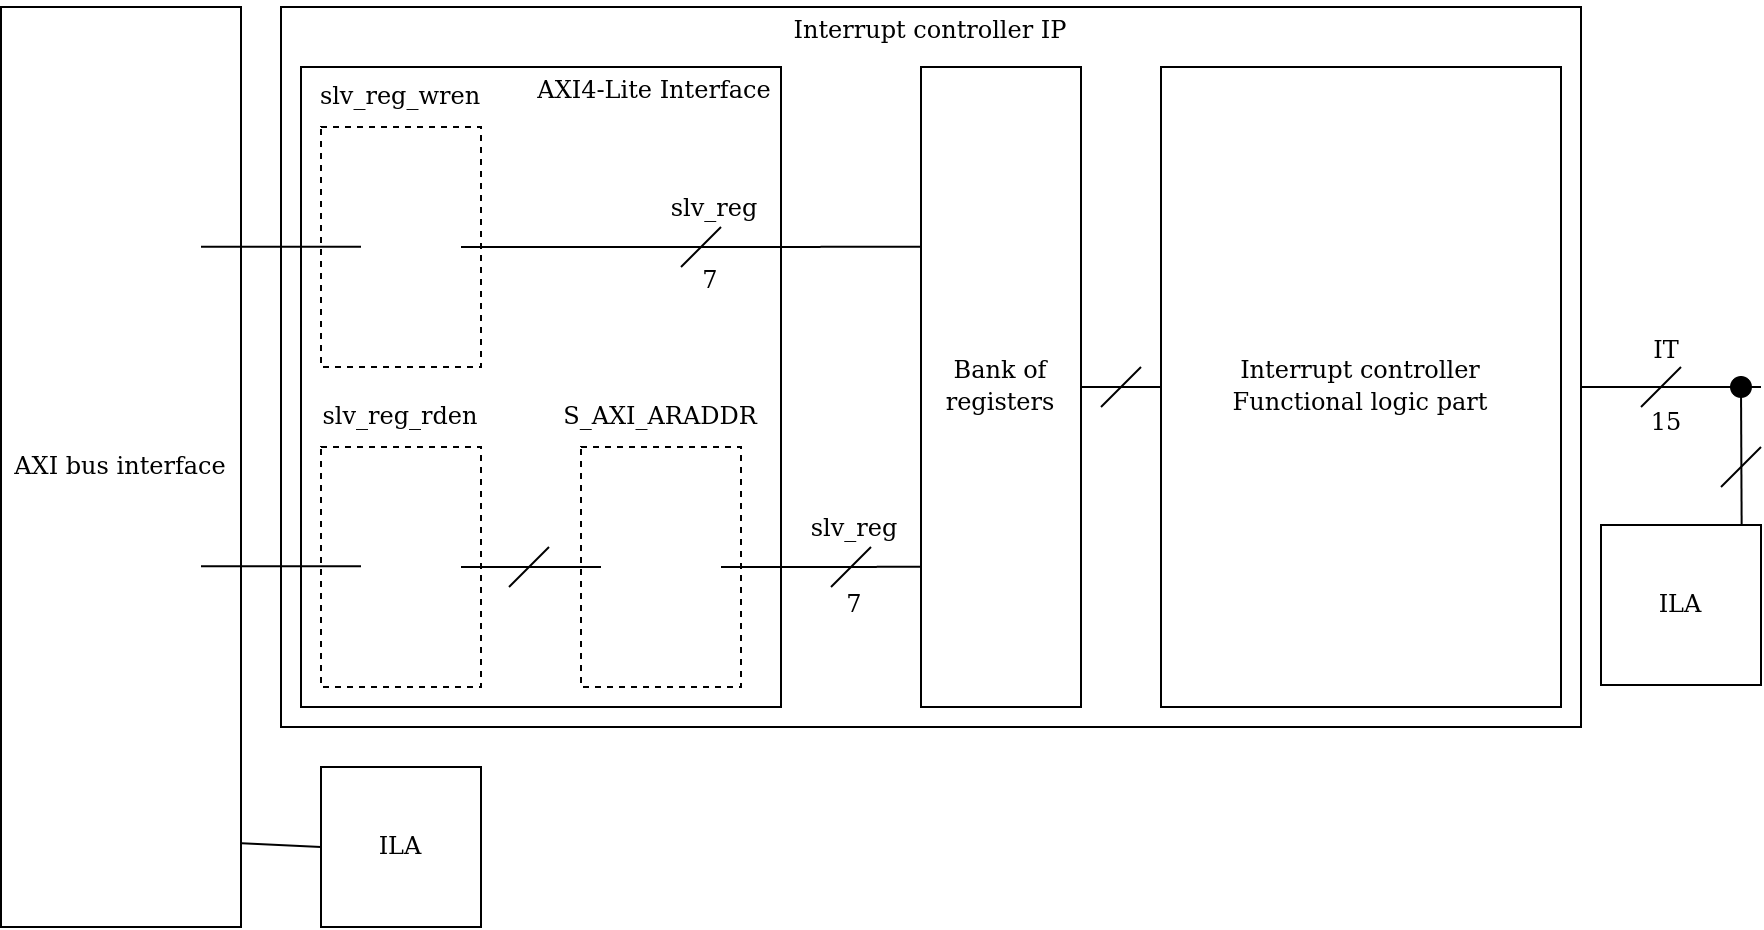
\includegraphics[width=0.8\linewidth]{figure/inside_IT_controller.png}
	\caption{Structure du contrôleur d'interruptions compatible AXI4-Lite}
	\label{fig:modif_IP}
\end{figure}
Le logiciel Vivado permet de générer une interface AXI configurable au sein de notre IP.
La structure générée comprend trois bloques internes assurant notamment le décodage des adresses.
Deux blocs ILA sont ajoutées sur la figure afin d'indiquer leur emplacement.
Ils ne serviront qu'à l'intégration et pourront être retirés par la suite.
